\appendices

\section{Architecture Modeling Details}

The main text only uses the architecture analysis to define system boundaries and time scales. The original architecture study follows a scenario-oriented model and simulation based system-of-systems engineering process. It treats vehicle-cloud collaborative tank-truck rollover prevention as a low-penetration highway mission in an intelligent vehicle cyber-physical system. The full architecture contains strategic, operational, service, and resource views. These views are useful for tracing requirements, but they are not necessary for the main algorithmic derivation.

The resulting design constraints used in this paper are as follows. First, the cloud side is an advisory and predictive layer rather than a direct actuator controller, and its main safety role is to reduce induced interaction risks before the ego vehicle enters a local emergency. Second, the vehicle side must maintain an independent safety loop because the cloud message may be delayed, lost, or invalidated by local perception. Third, the layered periods are approximately 1--2 Hz for cloud-side predictive planning, 10 Hz for vehicle-side emergency planning, and 20 Hz or higher for high-frequency anti-rollover control. Fourth, the emergency response chain must remain vehicle-side executable even when the cloud service is unavailable, so degraded safety does not rely on cloud availability.

\begin{figure}[t]
  \centering
  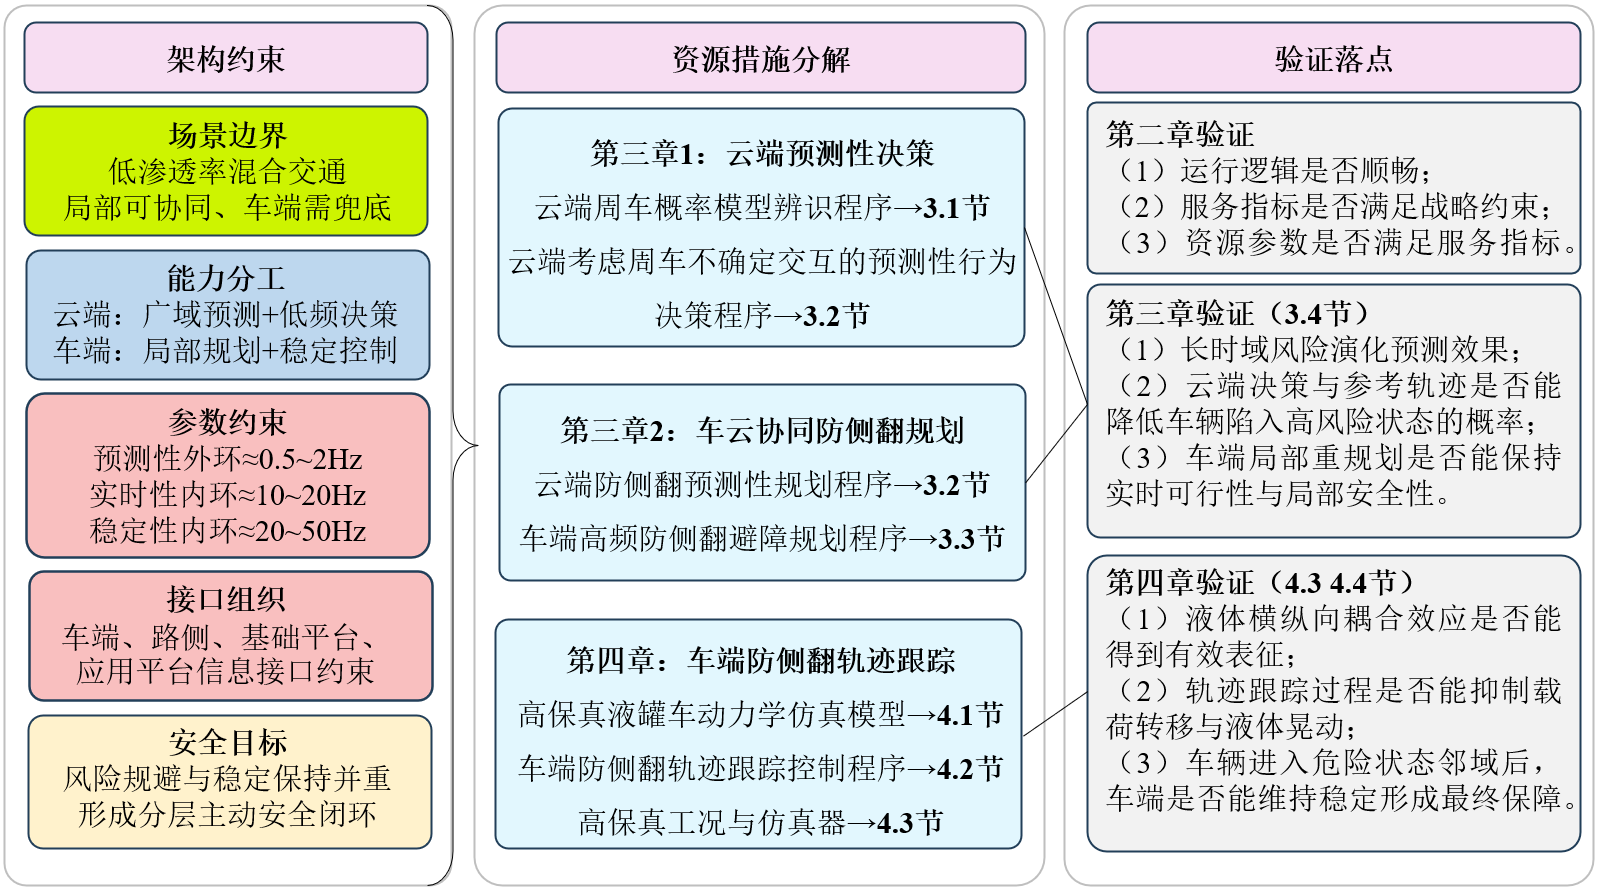
\includegraphics[width=0.95\linewidth]{fig/chap2/arch_method_mapping_v3.png}
  \caption{Traceability from architecture constraints to cloud-side planning, vehicle-side planning, and vehicle-side anti-rollover control.}
  \label{fig:appendix_arch_trace}
\end{figure}
% TODO: Redraw this appendix figure in English if the architecture traceability result is retained in the submitted manuscript.

\section{Graphflow Training and Decision Policy Details}

The Graphflow dataset is constructed by extracting a fixed road-graph region around the ego vehicle. The source implementation uses a forward range of about 700 m and a backward range of about 300 m to cover long-horizon highway interactions. Historical and future dynamic node features are mapped to the same graph topology, so autoregressive prediction can be performed by updating node features while keeping the edge set fixed.

The graph encoder uses three information sources: node features, edge features, and conditioning features. Node features describe static road semantics and dynamic traffic occupancy. Edge features describe road connectivity and lane-changing relations. Conditioning features include time encoding and ego action encoding. Local graph attention aggregates edge-aware neighbor information, while global attention captures long-range interaction over the graph. The output head predicts the dynamic-feature velocity field used in the flow-matching objective.

The reinforcement-learning decision policy uses a shared feature extractor for actor and critic. It encodes the traffic graph, ego features, and surrounding-vehicle historical features, then outputs an action sequence consisting of desired acceleration and lane-change command. The reward terms used in training are summarized in Table~\ref{tab:appendix_reward}.

\begin{table}[t]
  \centering
  \caption{Cloud-Side Policy Reward Terms}
  \label{tab:appendix_reward}
  \begin{tabularx}{\linewidth}{p{0.22\linewidth}X}
    \toprule
    Term & Role \\
    \midrule
    Safety & Penalizes ego occupancy on high graph-risk fields over the prediction horizon. \\
    Efficiency & Rewards speed close to road speed limits. \\
    Comfort & Penalizes acceleration magnitude and unnecessary lane changes. \\
    Consistency & Penalizes discontinuity between successive planned action sequences. \\
    Rule compliance & Penalizes speeding and unnecessary left-lane occupation. \\
    Navigation & Rewards staying on route-consistent graph nodes. \\
    \bottomrule
  \end{tabularx}
\end{table}

\section{Liquid-Sloshing Model Details}

The high-fidelity rapid sloshing model used in the thesis is the sliding telescopic libra model. It represents longitudinal-lateral coupled liquid motion through sliding lumped masses on smooth surfaces and curves. Compared with a two-dimensional pendulum model, this structure can describe liquid mass transfer between tank chambers, additional yaw moment induced by tank rotation, and longitudinal-lateral coupling under simultaneous acceleration, roll, and yaw excitation. The model was introduced to preserve the key six-degree-of-freedom sloshing modes needed by anti-rollover control while remaining much faster than CFD during repeated prediction.

The STL model can be written as
\begin{equation}
  [X_{STL}(k+1),Q_{STL}(k+1)]
  =f_{STL}(X_{STL}(k),u_l(k)|w_{STL}),
  \label{eq:appendix_stl}
\end{equation}
where $X_{STL}$ is the liquid-equivalent state, $u_l=[a_x,a_y,\phi,\ddot{\phi},\dot{\psi},\ddot{\psi}]^T$ is the tank excitation input, $w_{STL}$ is the identified parameter vector, and $Q_{STL}$ contains the equivalent liquid forces and moments. Parameters are identified from CFD data by minimizing the force/moment error over orthogonal excitation cases.

\begin{figure}[t]
  \centering
  \subfloat[STL model construction\label{fig:appendix_stl_model}]
    {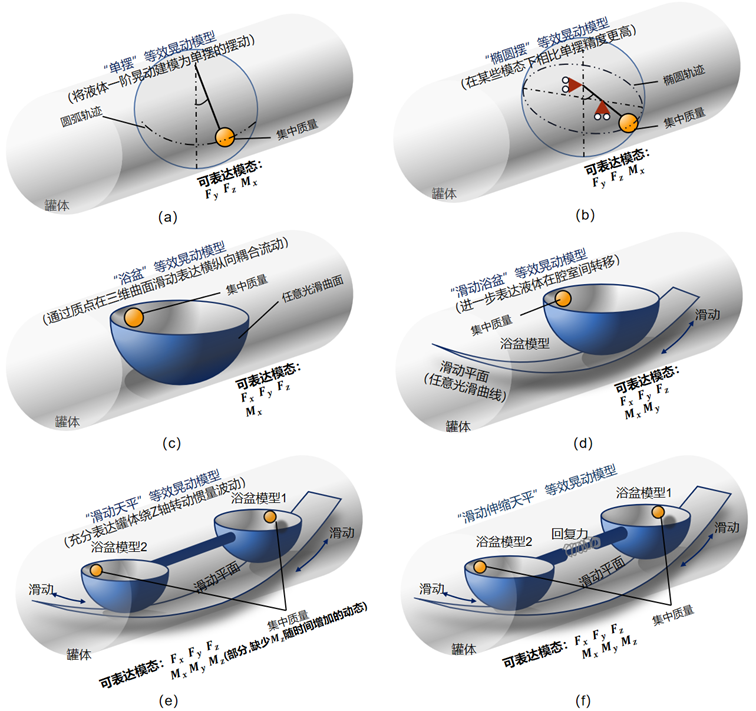
\includegraphics[width=0.95\linewidth]{fig/chap4/stl_model.png}}\\
  \subfloat[Residual re-linearization\label{fig:appendix_residual_learning}]
    {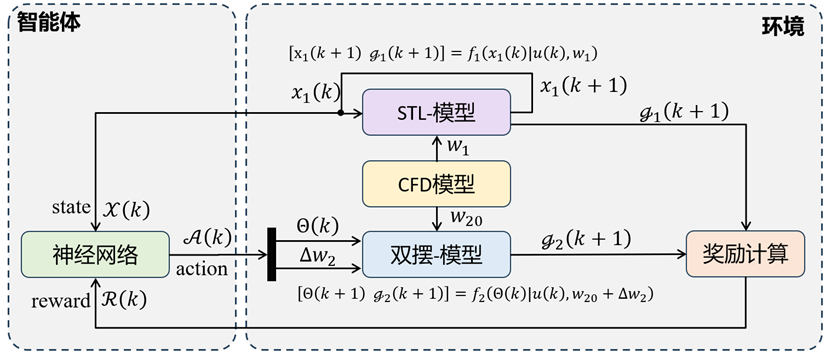
\includegraphics[width=0.95\linewidth]{fig/chap4/residual_learning.png}}
  \caption{Liquid-sloshing modeling and residual re-linearization.}
  \label{fig:appendix_liquid_model}
\end{figure}

For online MPC, the STL model is converted into a linearized double-pendulum model. A residual reinforcement-learning model maps the current STL state to parameter corrections and state estimates for the LDP model:
\begin{equation}
  [\Theta,\Delta w_{LDP}]=n_{\varphi}(X_{STL}),
  \label{eq:appendix_residual}
\end{equation}
where $\Theta$ is the LDP state estimate and $\Delta w_{LDP}$ is the parameter correction. The training reward penalizes the multi-step force/moment mismatch between STL and LDP outputs over representative excitations.

\section{Additional Validation and Platform Details}

The vehicle-liquid co-simulation platform couples TruckSim, Simulink, and StarCCM+. TruckSim provides vehicle acceleration and angular motion to the CFD model. StarCCM+ returns liquid forces and moments to the vehicle model. The data exchange interval in the reported co-simulation is 0.005 s. The liquid phase is gasoline-like $C_8H_{17}$ with 50\% filling ratio. The selected mesh setting is obtained from grid sensitivity analysis with average relative error below 1\% and peak error below 4\%.

The scaled experimental platform is a 1:14 semi-trailer model with an acrylic tank and anti-surge plates. The controller is implemented in C++ under ROS on a Jetson Orin NX. State measurements include IMU/GNSS pose and angular motion, wheel-encoder speed, and estimated liquid states. The similarity design uses static-stability-factor correction for vehicle rollover dynamics and Froude-number consistency for free-surface liquid sloshing. Additional experiment videos, simulation settings, and code-level implementation details are referenced in the thesis repository \cite{KomasaQi2026MasterThesis_repo}.
